\section{Tail mathematical model}
In order to devise a mathematical model of tail dynamics, we propose modeling the tail as a kinematic chain manipulator attached to robot body. Much like in aerial robots, when the robot is in the air, the tail acts frealy on its body. We propose using the tail as a dynamic stabilizator for the hopping. First we build the kinematic model using Denavit-Hartenberg parametrization metod, after that we devise a dynamic model of the arms using recursive Newton-Euler algorithm.

\subsection{Kinematic model}
Kinematic chain of the tail is shown in Fig. \ref{fig:rmax}, and the kinematic parameters are shown in table \ref{tab:DHParameters}. Kinematic chain consists of the body coordinate system, 2 revolute joints on of the tail, one virtual prismatic joint in the tail (i.e. Tail length parameter), and the tail tip coordinate system. As can be seen from DH parameters table, the two revolute joints have no linear, only angular dislacement from each other, therefore their masses and moments of inertia are all zero. The third prismatic joint represents the tail length and is modeled as a long stick with infitesimal thickness. 

\begin{table}
	\centering
		\begin{tabular}{ccccc}
		\hline
			& $\theta$ & $d$ & $a$ & $\alpha$ \\\hline
			\multicolumn{5}{c}{Body}\\\hline
			$B-0$ & $0$ & $d_B$ & $a_B$ & $0$\\\hline
			\multicolumn{5}{c}{Tail}\\\hline
			Joint 1 & $q_1$ & $0$ & $0$ & $-\frac{\pi}{2}$\\
			Joint 2 & $q_2$ & $0$ & $0$ & $\frac{\pi}{2}$\\
			Virtual joint& $0$ & $q_3$ & $0$ & $0$\\\hline
		\end{tabular}
	\caption{Denavit-Hartenberg Parameters}\label{tab:DHParameters}
\end{table}

\begin{equation}
T_0^3=\begin{bmatrix}
C_1 C_2 & -S_1 & C_1 S_2 & C_1 S_2 Q_3 \\
C_2 S_1 & C_1 & S_1 S_2 & S_1 S_2 Q_3 \\
-S_2 & 0 & C_2 & C_2 Q_3 \\
 0 & 0 & 0 & 1
\end{bmatrix}
\end{equation}

%\begin{multicols}{1}
\begin{equation}
\tau_b=\begin{bmatrix}
\frac{1}{24} m_3 Q_3 \left(-12 g S_1 S_2+Q_3 \left(3 S_1 S2_2 {\dot{Q}_1}^2-2 C_1\left(5+3 C2_2\right) \dot{Q}_1 \dot{Q}_2-3 C_1 S2_2 \ddot{Q}_1-8 S_1 \ddot{Q}_2\right)\right)\\
\frac{1}{24} m_3 Q_3 \left(-12 g C_1 S_2+Q_3 \left(S_1\left( 2(5+3C2_2)\dot{Q}_1 \dot{Q}_2+3S2_2\ddot{Q}_1\right)+C_1(3S2_2{\dot{Q}_1}^2-8\ddot{Q}_2)\right)\right)\\
\frac{1}{4} S_2 m_3 Q_3^2 \left(2 C_2 \dot{Q}_1 \dot{Q}_2+S_2 \ddot{Q}_1\right)
\end{bmatrix}
\end{equation}
%\end{multicols}

\begin{figure}
	\centering
	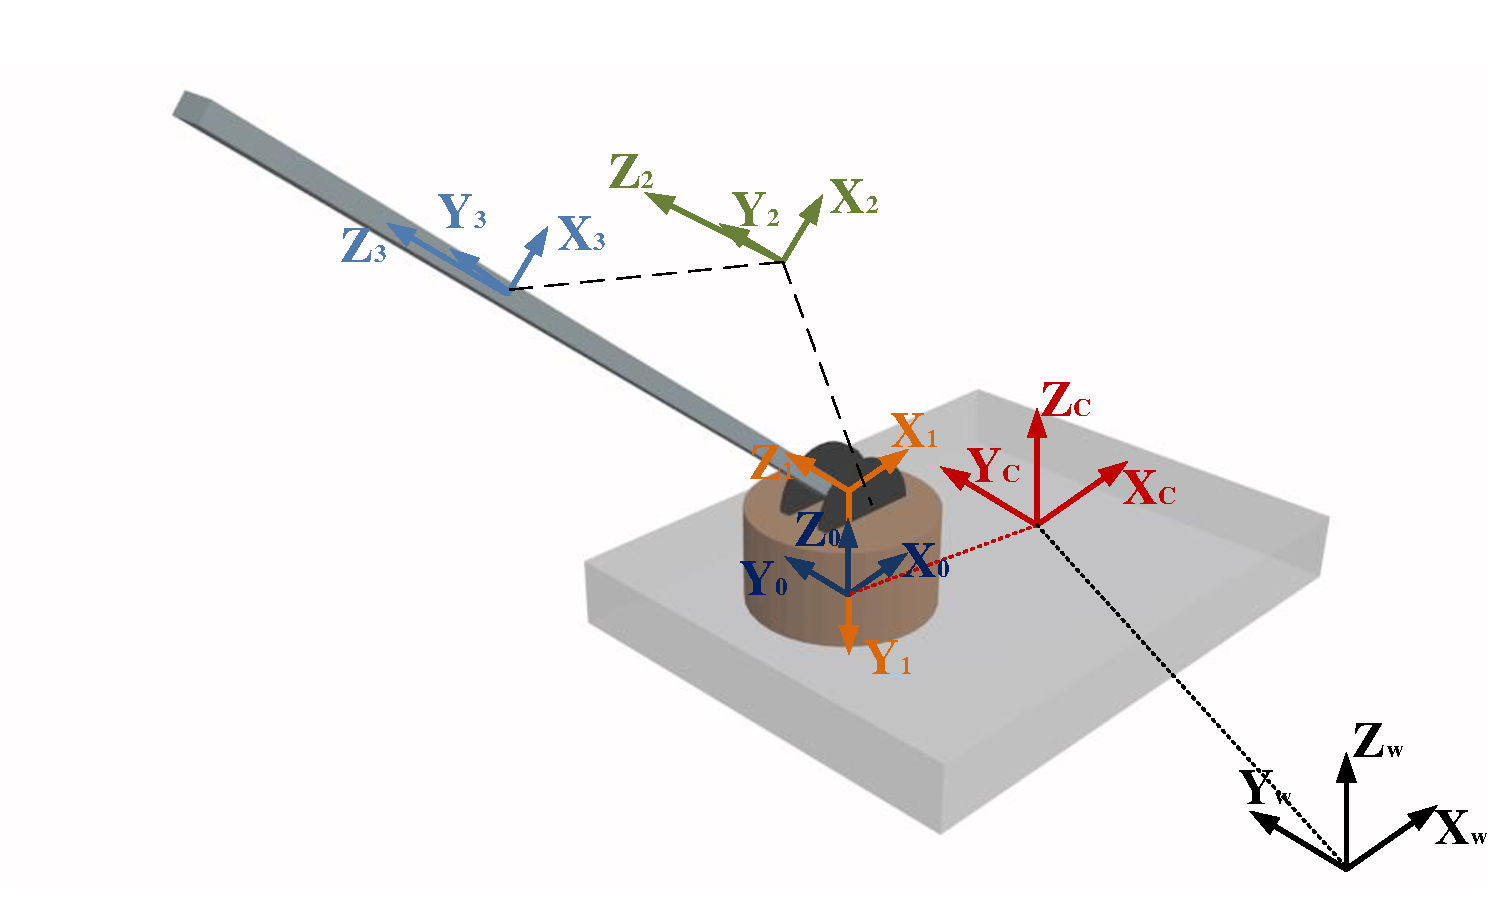
\includegraphics[width=85mm]{./pictures/RobinRepic.pdf}
	\caption{Robin Tail kinematic chain model}
	\label{fig:rmax}
\end{figure}

\subsection{Robin body}
In order to simplify the complexity of this analysis, we propose modeling Robin as a cuboid body, as shown in Fig \ref{fig:rmoment}. Moreover, Robin's body is a "container" for 4 cuboids, equaly displaced from the body center. Ideally, when Robin's body is fully simetric, all four cuboids have the same mass. Since in most situations this is not the case, each cuboid has its own mass $m_i$, its own center of mass $cm_i$ placed in its center, and $\vec{r}_i$, the distance between the $cm_i$ and the body coordinate system. The overall center of mass is then easily calculated from: 
\begin{equation}
CM=\frac{\sum_{i=1}^{4}m_i\vec{r}_i}{\sum_{i=1}^{4}m_i}
\end{equation}
Next important dynamic parameter is the moment of inertia tensor. Having for cuboid bodys as the basis of robot body model, tensor of inertia can easily be derived by using the Parallel axis theorem:
\begin{equation}
J_R=\sum_{i=1}^{4}\left \{J_{c_i}+m_i\begin{bmatrix}
{_yr_i}^2+{_zr_i}^2 & {_xr_i}\cdot {_yr_i} & {_xr_i}\cdot {_zr_i} \\ 
-{_xr_i}\cdot {_yr_i} & {_xr_i}^2+{_zr_i}^2 & {_yr_i}\cdot {_zr_i}\\ 
-{_xr_i}\cdot {_zr_i} & {_yr_i}\cdot {_zr_i} & {_yr_i}^2+{_xr_i}^2
\end{bmatrix} \right \}
\end{equation}

where, $_xr_i, _yr_i, _zr_i$ represent $\vec{r}_i$ projection in $x,y,z$ respectively, and $J_{c_i}$ is the moment of inertia of the single cuboid element of height $h_i$, width $w_i$ and length $l_i$:
\begin{equation}
J_{c_i}=\frac{m_i}{12}\begin{bmatrix}
w_i^2+d_i^2 &0&0 \\ 
0 &h_i^2+d_i^2&0\\ 
0 &0& w_i^2+h_i^2
\end{bmatrix}
\end{equation} 

It could be easily shown that if all four cuboids have the same mass and size (i.e. $m,h,d,w$) and are simetrically displaced from the body center, as shown in Fig \ref{fig:rmoment}, the total body moment of inertira $J_R$ comes down to a symetric matrix:
\begin{equation}
J_{c_i}=\frac{m}{12}\begin{bmatrix}
(2w)^2+d^2 &0&0 \\ 
0 &(2h)^2+d^2&0\\ 
0 &0& (2w)^2+(2h)^2
\end{bmatrix}
\end{equation} 
and the body center of mass is placed directly in the center of body coordinate system. For any other arrangment, tensor matrix will not be symmetric, and what is even worse, the body center of mass will be missaligned.

Acting as an active spring, while quadriped is hoping, each leg excerts force on its body. The legs are positioned symetrically around the geometric center, and similarly as quadrotor aircraft produce the following forces and torques:

\begin{gather}\label{eq:Forces}
\vec{F_{tot}}=\sum_{i=1}^{4}(\vec{T_{i}}+\vec{S_{i}})\\
\vec{\tau_{tot}}=\sum_{i=1}^{4}\vec{\rho _i}(\vec{T_{i}}+\vec{S_{i}})
\end{gather}  

Where $\vec{T_{i}}$ represents the $i$-th cuboid thrust force that causes vertical movement (i.e. hopping), $\vec{S_{i}}$ $i$-th cuboid side force that moves the qudriped in x direction, and $\rho _i$ $i$-th distance between the geometric center and forces.

\begin{figure}
	\centering
	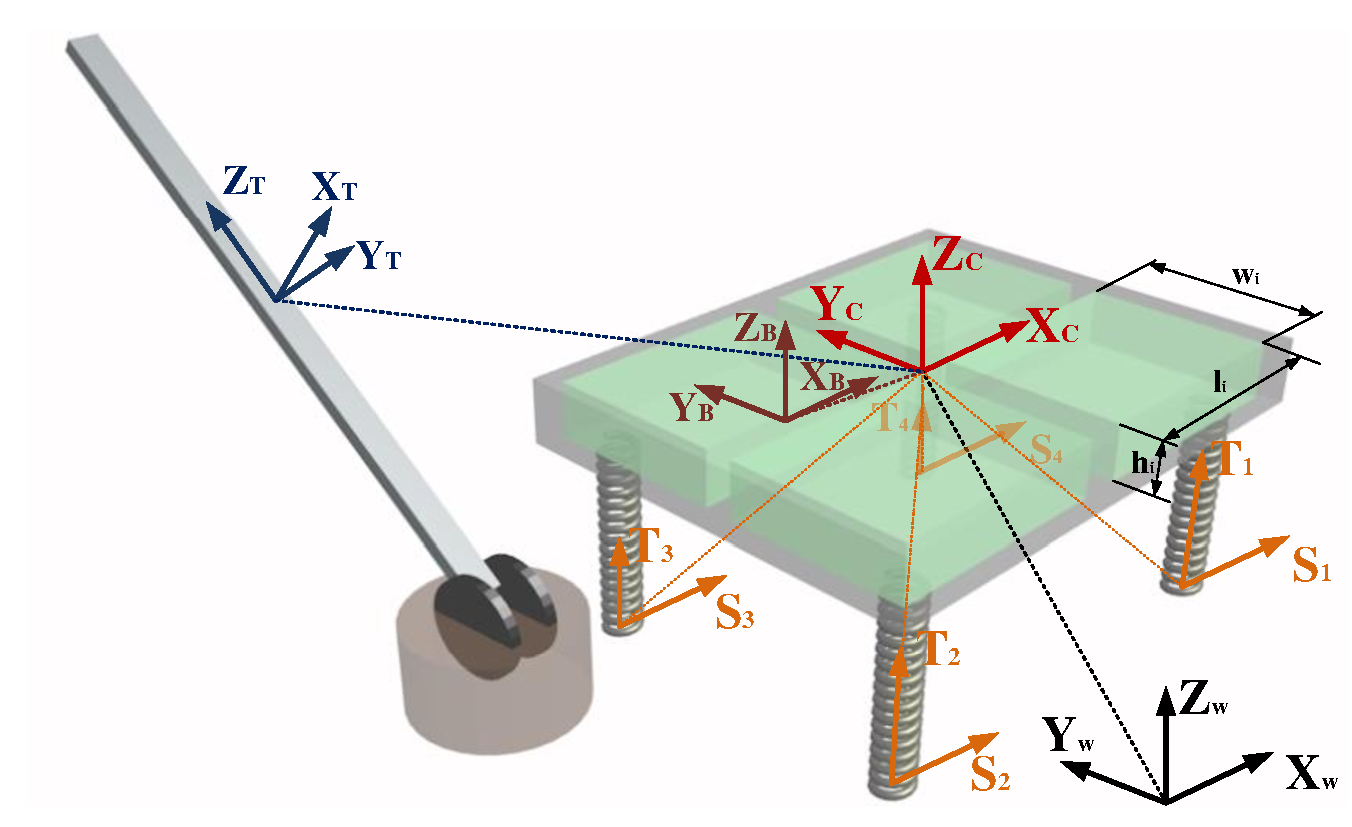
\includegraphics[width=85mm]{./pictures/RobinMoment.pdf}
	\caption{Robin body dynamics}
	\label{fig:rmoment}
\end{figure}

\subsection{Tail dynamics}
In Fig. \ref{fig:rmoment}, tail coordinate system is depicted. Due to the tail's infitesimal thickness, its moment of inertia, written in this frame is:

\begin{equation}
J_3=\frac{{Q_3}^2 m_3}{12}\left(
\begin{array}{ccc}
 1 & 0 & 0 \\
 0 & 1 & 0 \\
 0 & 0 & 0
\end{array}
\right)
\end{equation} 

